

\documentclass[10pt]{beamer}
\usepackage{amsmath,amssymb}
\usepackage[brazil]{varioref}
\usepackage[russian,english]{babel}
\usepackage[utf8]{inputenc}
\usetheme{default}
\usepackage{mathtools}
\usepackage{multirow}
\mathtoolsset{showonlyrefs}



\definecolor{cvut_navy}{HTML}{0065BD}
\definecolor{cvut_blue}{HTML}{6AADE4}
\definecolor{cvut_gray}{HTML}{156570}

% \setbeamercolor{section in toc}{fg=black,bg=white}
% \setbeamercolor{alerted text}{fg=cvut_blue}
% \setbeamercolor*{palette primary}{bg=cvut_navy,fg=gray!20!white}
% \setbeamercolor*{palette secondary}{bg=cvut_blue,fg=white}
% \setbeamercolor*{palette tertiary}{parent=palette primary}
% \setbeamercolor*{palette quaternary}{fg=green,bg=gray!5!white}

% \setbeamercolor*{sidebar}{fg=cvut_navy,bg=gray!15!white}


% \setbeamercolor{titlelike}{parent=palette primary}
% \setbeamercolor{frametitle}{parent=palette primary}

% \setbeamercolor*{separation line}{}
% \setbeamercolor*{fine separation line}{}

\setbeamertemplate{navigation symbols}{} 


\usepackage{amsmath, amssymb, amsfonts}
\usepackage[utf8]{inputenc}
\usepackage{movie15}
\usepackage[T2A]{fontenc}
\usepackage{graphicx}
\usepackage{subfig}
\usepackage[noend]{algorithmic}
\usepackage{tikz}
\usepackage{amsmath,amsfonts,amsthm,amssymb,amsbsy,amstext,amscd,amsxtra,multicol}
\usepackage{verbatim}
\usetikzlibrary{automata,positioning}
\usepackage{multicol}
\usepackage{graphicx}


\usepackage{appendixnumberbeamer}
%\usecolortheme{dove}
%\usefonttheme{serif}

\newcommand{\cond}{\mspace{3mu}{|}\mspace{3mu}}
\newcommand{\norm}{\mathop{\rm norm}\limits}
\newcommand{\tsum}{\mathop{\textstyle\sum}\limits}
\newcommand{\tprod}{\mathop{\textstyle\prod}\limits}

\let\l\limits


\title
[Слайд \hfill\insertframenumber\,/\,\inserttotalframenumber ]
{\largef Parseval’s Theorem \\and\\ 
Fourier Inversion Theorem}
\author[Student Filipp Nikitin]{%
  Student Filipp Nikitin
  }
  \institute[MIPT]{
      Moscow institute of Physics and Technology
\\(state university)\\
     Phystech school of applied mathematics and informatics
     }
\date{\today}

\begin{document}

\begin{frame}
    \titlepage
    \begin{center}
          
\includegraphics[height=1.4cm]{logo_img/mipt.png} \ \ \
        
\includegraphics[height=1.4cm]{logo_img/vc-ran_logo.png}
    \end{center}
\end{frame}

\begin{frame}[t]{Plan}

\begin{enumerate}
    \item Introduction
    
    \item Fourier Transforms

    \item Fourier Inversion Theorem 
    
    \item Fourier Inversion Theorem(proof)
    
    \item Parseval’s Theorem
    
    \item Parseval’s Theorem(proof)
    
    \item Discussion
    
    
    
\end{enumerate}
    
\end{frame}


\begin{frame}[t]{Time and Frequency Domains}

Two ways of process descibing:

\begin{itemize}
    \item \textbf{Time domain}. Values of some quantity
    
    \item \textbf{Frequency Domain}. Complex number: amplitude and phase 
\end{itemize}

\begin{block}{Fourier transforms}
The mapping between the domains
\end{block}

    \begin{figure}
        \centering
        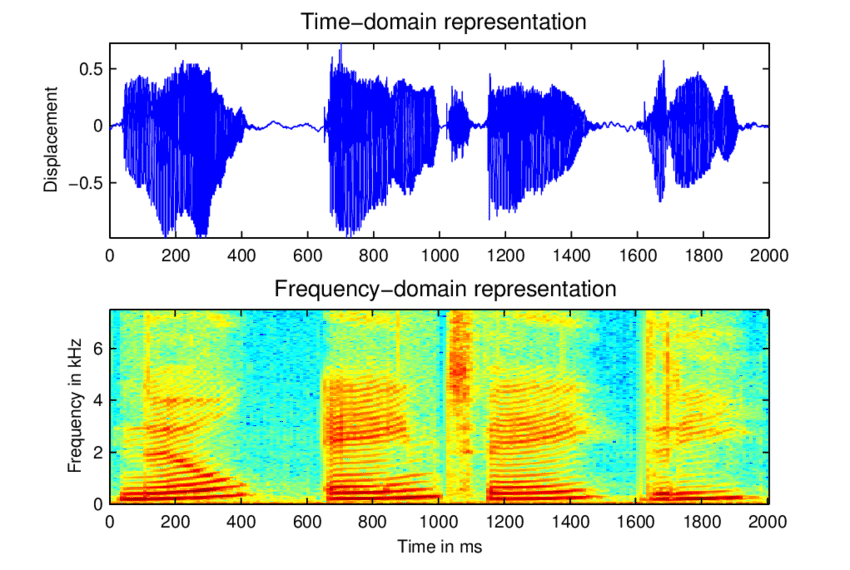
\includegraphics[width=.7\textwidth]{domains.png}
        \caption{Two representations of speech.}
    \end{figure}

\end{frame}


\begin{frame}{Fourier Inversion Theorem}

\begin{enumerate}
    \item From time domain to frequency domain:
    \begin{equation}
        H(f) = \int \limits_{-\infty}^{+\infty} h(t) \exp({- ift}) dt 
    \end{equation}
    
    \item From frequency domain to time domain:
    \begin{equation}
        h(t) = \frac{1}{2\pi}\int \limits_{-\infty}^{+\infty} H(f) \exp({ ift}) df
    \end{equation}
\end{enumerate}


\begin{block}{Properties}
\begin{enumerate}
    \item FT is a linear operator
    \item Time scaling: $h(at) \equiv \frac{1}{a}H(\frac{f}{a})$
    \item Time shifting: $h(t-t_0) \equiv H(f) \exp(- ift_0)$ 
\end{enumerate}

\end{block}

    
\end{frame}


\begin{frame}{Fourier Inversion Theorem(proof)}

\begin{block}{Assume}
    \begin{align}
        H(f) &=  A \int \limits_{-\infty}^{+\infty} h(t) \exp({- ift}) dt  \\
        h(t) &= B \int \limits_{-\infty}^{+\infty} H(f) \exp({ ift}) df
    \end{align}
\end{block}
    
\begin{block}{When}
    \begin{align}
        h(t) &= AB \int \limits_{-\infty}^{+\infty} A \int \limits_{-\infty}^{+\infty} h(\tau) \exp({- if\tau}) \exp({ ift}) d\tau df = \\
        &= \int \limits_{-\infty}^{+\infty} \left[ AB \int \limits_{-\infty}^{+\infty} \exp({- if\tau}) \exp({ ift}) df \right]\; h(\tau) d\tau
    \end{align}
\end{block}

\end{frame}

\begin{frame}{Fourier Inversion Theorem(proof)}
\block{QM flashback}
\begin{equation}
    AB \int \limits_{-\infty}^{+\infty} \exp({- if\tau}) \exp({ ift}) df = \delta (t - \tau)
\end{equation}
\end{block}
where $\delta$ is a Dirac Delta function


\begin{block}{When}
    \begin{align}
        AB & \int \limits_a^b \int \limits_{-\infty}^{+\infty}  \exp({ if(t - \tau)}) df d(t-\tau) = \frac{\text{sign(b)} - \text{sign(a) }}{2} = \\
        &=   AB \int \limits_a^b \int \limits_{0}^{+\infty}  \exp({ ify}) + \exp({ -ify} ) df dy = \\
        &4AB \int \limits_{0}^{+\infty} \int \limits_a^b cos(ky) dy \; d\tau = \text{sign}(b) - \text{sign}(a)
    \end{align}
\end{block}

\end{frame}


\begin{frame}{Fourier Inversion Theorem(proof)}

\begin{align}
4AB \int \limits_{0}^{+\infty} \int \limits_a^b cos(\tau y) dy \; d\tau =   4AB \int \limits_{0}^{+\infty} \frac{\sin(\tau b) - \sin(\tau a)}{\tau} d \tau
\end{align}


\begin{block}{Dirichlet integral}
\begin{equation}
    \int \limits_{0}^{+\infty} \frac{\sin{u}}{u} du = \frac{1}{4AB};\ AB = \frac{1}{\pi}
\end{equation}
\end{block}

\end{frame}


\begin{frame}{Parseval’s Theorem }

\begin{block}{Theorem}
\begin{equation}
        \frac{1}{\pi} \int \limits_{-\infty}^{+\infty} |H(f)|^2 df = \int \limits_{-\infty}^{+\infty} |h(t)|^2 df 
\end{equation}
\end{block}


\begin{block}{General Form(Plancherel’s formula)}
\begin{equation}
        \frac{1}{2\pi} \int \limits_{-\infty}^{+\infty} H(f)G^*(f) df = \int \limits_{-\infty}^{+\infty} h(t) g^*(t) dt
\end{equation}
\end{block}
\end{frame}


\begin{frame}{Plancherel’s formula(proof)}

\begin{block}{Proven statement}
\begin{equation}
    \delta(x) = \frac{1}{2\pi} \int \limits_{-\infty}^{+\infty} exp(ixt)dt
\end{equation}

\end{block}

\begin{block}{When}
    \begin{align}
        &\int \limits_{-\infty}^{+\infty} h(t) g^*(t) df  =\\ 
        &\int \limits_{-\infty}^{+\infty} \left(\frac{1}{2\pi} \int \limits_{-\infty}^{+\infty} H(f) \exp(ift)df \right) \left(\frac{1}{2\pi} \int \limits_{-\infty}^{+\infty} G^*(f') \exp(if't)df' \right)dt  = 
    \end{align}
\end{block}

\end{frame}



\begin{frame}{Plancherel’s formula(proof)}

\begin{align}
&\int \limits_{-\infty}^{+\infty} \left(\frac{1}{2\pi} \int \limits_{-\infty}^{+\infty} H(f) \exp(ift)df \right) \left(\frac{1}{2\pi} \int \limits_{-\infty}^{+\infty} G^*(f') \exp(if't)df' \right)dt  = \\
& \frac{1}{4\pi^2} \int \limits_{-\infty}^{+\infty} \int \limits_{-\infty}^{+\infty} H(f) G^*(f') \int \limits_{-\infty}^{+\infty} \left(\exp(i(f - f')t) dt\right)\; df\; df'\; = \\
& \frac{1}{2\pi} \int \limits_{-\infty}^{+\infty} \int \limits_{-\infty}^{+\infty} H(f) G^*(f')  \delta(f - f')\; df\; df'\; =  \frac{1}{2\pi} \int \limits_{-\infty}^{+\infty} H(f)G^*(f) df
\end{align}

\begin{block}{Note}
Taking $h \equiv g$  we immediately obtain Parseval’s Theorem
\end{block}

\end{frame}


\begin{frame}{Summary}
\begin{itemize}
    \item Introduction
    
    \item Fourier Transforms

    \item Fourier Inversion Theorem 
    
    \item Fourier Inversion Theorem(proof)
    
    \item Parseval’s Theorem
    
    \item Parseval’s Theorem(proof)
    
    \item Discussion
\end{itemize}
\end{frame}




\begin{frame}
\centering
\Large{Thank you!}
\end{frame}



{\small
\begin{frame}[allowframebreaks]{Основная литература}
    \bibliographystyle{plainnat}
    \nocite{*}
    \bibliography{demo}    
\end{frame}
}



\end{document}
